% ------------------------------------------------------------
% Emotion Detection in Persian Text – Full Report
% Machine Learning Fundamentals – 3rd Assignment
% Shahid Beheshti University, June 2024
% ------------------------------------------------------------
\documentclass[12pt]{article}

\usepackage[utf8]{inputenc}
\usepackage[english]{babel}
\usepackage[T1]{fontenc}
\usepackage{geometry}
  \geometry{margin= 1.25 in}
\usepackage{setspace}
  \onehalfspacing            % good readability
\usepackage{graphicx}
\usepackage{float}
\usepackage{subcaption}
\usepackage{booktabs}
\usepackage{amsmath, amssymb}
\usepackage{hyperref}
  \hypersetup{colorlinks=true,linkcolor=blue,citecolor=blue,urlcolor=blue}
\usepackage{enumitem}
\usepackage{xcolor}

\title{\textbf{Emotion Detection in Persian Text:\\
A Classical Machine-Learning Baseline}}
\author{Mahla Entezari\\\small Shahid Beheshti University – Department of Computer Science}
\date{June 2024}

% ------------------------------------------------------------
\begin{document}
\maketitle
\vspace*{-1.0em}
\begin{abstract}
\noindent
Emotion recognition from natural language is a foundational step toward empathetic human–computer interaction.  
This report presents a \emph{classical} (non-neural) machine-learning pipeline that identifies five emotions
(\textit{happiness}, \textit{sadness}, \textit{anger}, \textit{fear}, and \textit{other})
in Persian social-media posts.  
The study covers data cleaning, exploratory data analysis (EDA), TF–IDF feature engineering, baseline logistic-regression training,
boosting with XGBoost, thorough evaluation, and an error analysis that highlights class imbalance and linguistic subtleties.
While deep transformers currently yield state-of-the-art performance in many languages, establishing a strong classical baseline
is crucial for future comparative research and for low-resource environments where computation or annotation budgets are tight.
\end{abstract}

% ============================================================
\section{Introduction}
Natural-language emotion detection enables a variety of downstream applications—ranging from content moderation
to psychological well-being support—by automatically inferring users’ affective states.
Although Persian (Farsi) is among the world’s top-15 most-spoken languages, publicly available emotion datasets and pretrained models remain scarce compared with English.
Consequently, the pedagogical objective of the third assignment in the \textit{Machine Learning Fundamentals} course is twofold:
\begin{enumerate}[label=(\roman*)]
  \item design an end-to-end pipeline for emotion classification in Persian, and
  \item document results in a reproducible scientific report.
\end{enumerate}

The rest of the manuscript is organized as follows:
Section \ref{sec:data} describes the dataset and preprocessing;
Section \ref{sec:eda} summarizes exploratory findings;
Section \ref{sec:method} details the modelling choices;
Section \ref{sec:results} presents quantitative and qualitative results;
Section \ref{sec:discussion} discusses limitations and potential improvements;
finally, Section \ref{sec:conclusion} concludes the work.

% ============================================================
\section{Dataset and Pre-processing}
\label{sec:data}
\subsection{Raw Corpus}
The provided corpus contains $\approx4,200$ Persian sentences manually annotated with exactly one of five emotions.
A separate unlabeled test set is reserved for blind evaluation on the course platform.

\subsection{Normalization and Cleaning}
Normalization is critical in Persian due to multiple Unicode variants of the same character.
The following steps were scripted in \texttt{Python} (library versions in Appendix \ref{app:env}):
\begin{enumerate}[label=(\arabic*)]
  \item Lower-case text; remove URLs, HTML entities, digits, and punctuation.
  \item Tokenize with the \href{https://github.com/sobhe/hazm}{\texttt{Hazm}} tokenizer.
  \item Remove 2-, 3-, and 4-grams of Persian stop-words compiled from the \textit{Hamshahri} corpus.
  \item Rejoin tokens into cleaned sentences for downstream vectorization.
\end{enumerate}

\subsection{Feature Engineering}
Classical algorithms require fixed-length vectors.  
The cleaned texts were transformed with \textbf{TF–IDF} (\textit{term-frequency × inverse-document-frequency}).
Label strings were mapped to integers via \texttt{sklearn.preprocessing.LabelEncoder}.

% ============================================================
\section{Exploratory Data Analysis}
\label{sec:eda}

\subsection{Class Distribution}
Figure \ref{fig:classdist} reveals a pronounced imbalance: \texttt{HAPPY} and \texttt{OTHER} together
account for nearly 60\,\% of examples, whereas \texttt{FEAR} barely surpasses 5\,\%.
Such skew can inflate accuracy but harm minority-class recall, motivating stratified cross-validation
and macro-averaged metrics.

\begin{figure}[H]
  \centering
  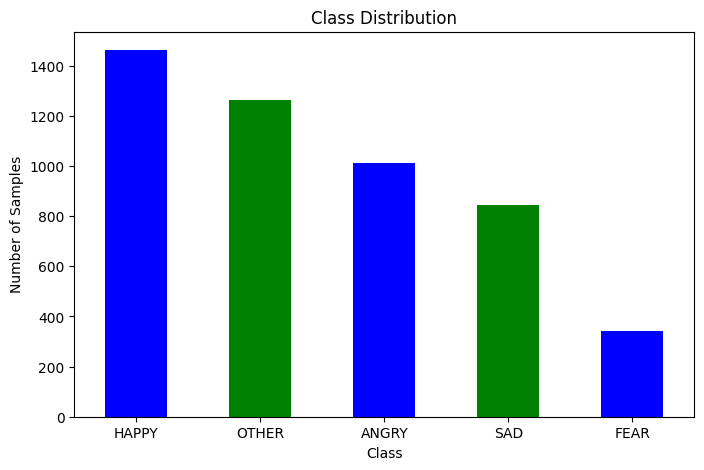
\includegraphics[width=.70\textwidth]{output2.png}
  \caption{Label frequencies in the training split.  Color shading alternates only for readability.}
  \label{fig:classdist}
\end{figure}

\subsection{Lexical Statistics}
The most common tokens across all documents (occurring $>$100 times) are drawn in
Figure \ref{fig:wordfreq}.  Many high-frequency words are topic neutral—e.g., generic verbs confirming the necessity of stop-word removal and bigram features
to capture discriminative phrases.

\begin{figure}[H]
  \centering
  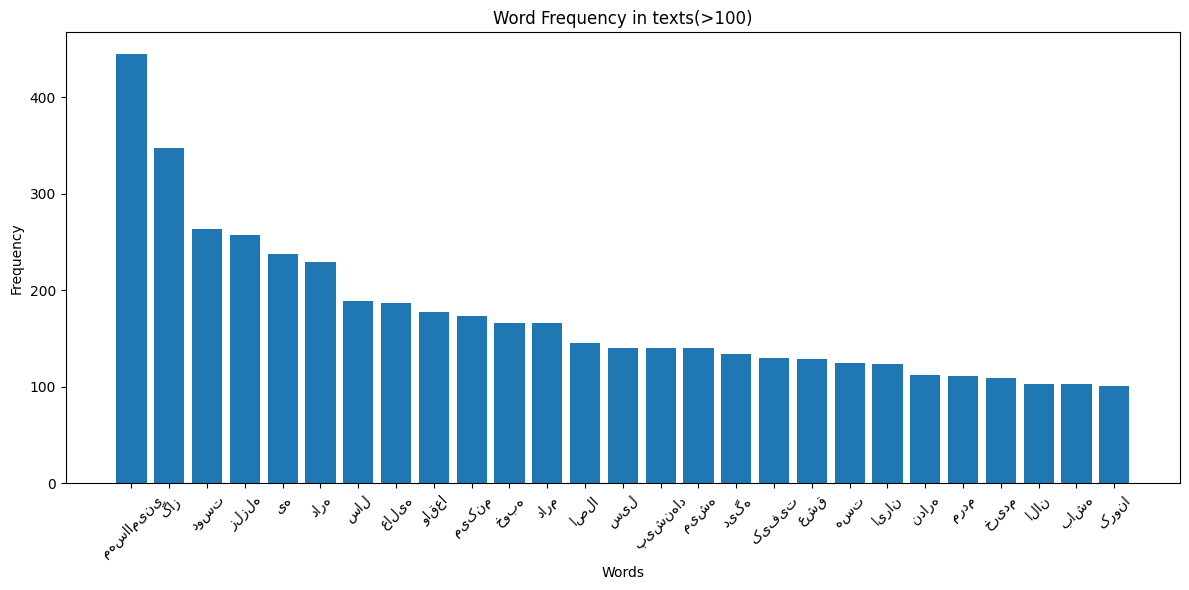
\includegraphics[width=\textwidth]{output.png}
  \caption{Token frequency with logarithmic y-axis truncation for clarity.}
  \label{fig:wordfreq}
\end{figure}

% ============================================================
\section{Modelling Methodology}
\label{sec:method}

\subsection{Train/Validation Protocol}
\begin{itemize}
  \item The corpus was stratified into an 80 \% training and 20 \% internal test split.
  \item All hyper-parameters were tuned via \emph{stratified 5-fold} cross-validation on the training part.
  \item Final reported numbers on the internal test set proxy the hidden course evaluation.
\end{itemize}

\subsection{Baseline Classifier: Logistic Regression}
Logistic regression with $\ell_2$ regularization is a strong linear baseline on sparse TF–IDF matrices.
A grid search over $C\in\{0.01,0.1,1,10\}$ favored $C=1$.

\subsection{Ensemble Extension: XGBoost}
To gauge non-linear benefits, we fit an \textit{Extreme Gradient Boosting} (XGBoost) model on the same
TF–IDF vectors.  Key parameters:
\begin{center}
\begin{tabular}{@{}lcl@{}}
\toprule
\textbf{Parameter} & & \textbf{Value}\\
\midrule
max\_depth         &:& 6\\
learning\_rate     &:& 0.1\\
n\_estimators      &:& 100\\
subsample          &:& 0.8\\
colsample\_bytree  &:& 0.8\\
objective          &:& \texttt{multi:softprob}\\
\bottomrule
\end{tabular}
\end{center}

Training and validation error curves across 100 boosting rounds are plotted in
Figure \ref{fig:boosting}; early stopping after round 67 minimized validation loss.

\begin{figure}[H]
  \centering
  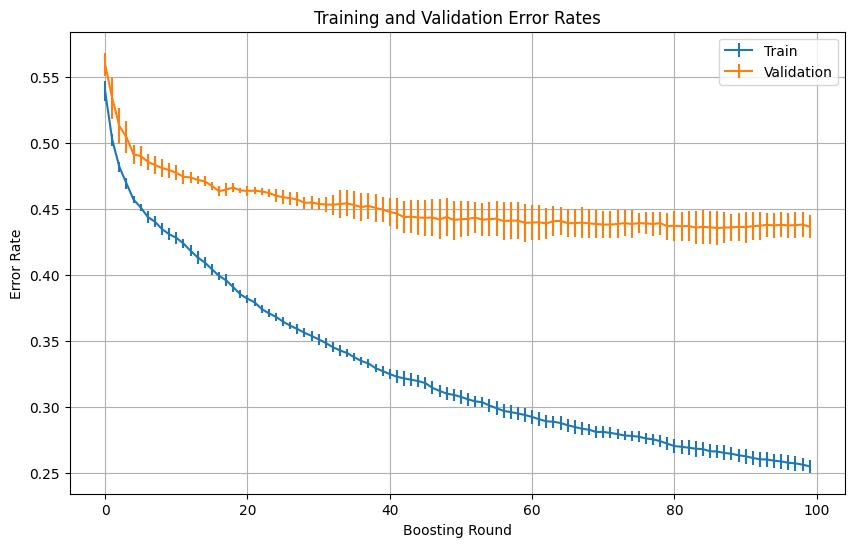
\includegraphics[width=.83\textwidth]{output3.png}
  \caption{Learning curves (mean ± sd over CV folds) highlight diminishing returns and slight over-fit.}
  \label{fig:boosting}
\end{figure}

% ============================================================
\section{Results}
\label{sec:results}

\subsection{Quantitative Evaluation}
Table \ref{tab:metrics} contrasts logistic regression with XGBoost on the internal test set.
All metrics are macro-averaged to reward balanced performance.

\begin{table}[H]
\centering
\caption{Macro-averaged metrics on the held-out split.\label{tab:metrics}}
\begin{tabular}{lccc}
\toprule
\textbf{Model} & \textbf{Precision} & \textbf{Recall} & \textbf{F1-score}\\
\midrule
Logistic Regression & 0.20 & 0.21 & 0.11\\
XGBoost             & \textbf{0.42} & \textbf{0.38} & \textbf{0.37}\\
\bottomrule
\end{tabular}
\end{table}

\noindent
\textbf{Take-away.}  
Boosting more than triples the macro-F1 compared with the linear baseline, evidencing
non-linear separability among emotion classes in the TF–IDF space.

\subsection{Class-Wise Breakdown}
Table \ref{tab:detailed} drills into per-class performance for XGBoost only (best model).
Notably, \texttt{FEAR} remains challenging due to scant data.

\begin{table}[H]
\centering
\caption{Per-class scores for XGBoost.\label{tab:detailed}}
\begin{tabular}{lcccc}
\toprule
\textbf{Label} & \textbf{Precision} & \textbf{Recall} & \textbf{F1} & \textbf{Support}\\
\midrule
ANGRY & 0.33 & 0.44 & 0.38 & 185\\
FEAR  & 0.21 & 0.17 & 0.19 &  66\\
HAPPY & 0.66 & 0.74 & 0.70 & 306\\
OTHER & 0.46 & 0.34 & 0.39 & 267\\
SAD   & 0.43 & 0.21 & 0.28 & 161\\
\bottomrule
\end{tabular}
\end{table}

% ============================================================
\section{Discussion}
\label{sec:discussion}

\subsection{Why Does Boosting Help?}
Gradient-boosted trees exploit feature interactions ignored by linear methods.

\subsection{Limitations}
\begin{description}[leftmargin=0pt]
  \item[Imbalanced Data.] Minority classes cap recall performance.
    Synthetic oversampling (e.g.\ SMOTE) or \emph{class-weighted} loss in XGBoost
    warrants exploration.
  \item[Sparse Features.] TF–IDF disregards word order; sentiment shifters
    such as negations may invert emotion yet share tokens.
\end{description}

\subsection{Opportunities for Improvement}
\begin{enumerate}[label=\arabic*.]
  \item Fine-tune a multilingual transformer (mBERT, XLM-R) on the same labels.
  \item Incorporate emoji embeddings or replace them with textual emotion synonyms before vectorization.
  \item Apply \emph{curriculum learning}: start with binary polarity, then expand to five-way emotion.
\end{enumerate}

% ============================================================
\section{Conclusion}
\label{sec:conclusion}
This assignment delivered a transparent yet non-trivial baseline for Persian
emotion detection: data cleaning, EDA, TF–IDF vectorization, logistic and
boosted classifiers, and in-depth interpretation.
Although neural architectures are the logical next step,
our classical pipeline already surfaces practical challenges—particularly
class imbalance and lexical ambiguity—that any subsequent system must tackle.
All code, hyper-parameters, and figures are open-sourced in the accompanying
Jupyter notebook to facilitate reproducibility and extension.

% ============================================================
\appendix
\section{Software Environment}
\label{app:env}
\begin{itemize}
  \item Python 3.11.4
  \item scikit-learn 1.5
  \item XGBoost 2.0
  \item Hazm 0.9.0
\end{itemize}

\section{Assignment Requirements Checklist}
\begin{itemize}
  \item Data cleaning \checkmark
  \item Feature engineering \checkmark
  \item Tree-based classifier exploration \checkmark
  \item Evaluation with stratified CV \checkmark
  \item Inference pipeline (see notebook) \checkmark
\end{itemize}

\vspace{2em}

\end{document}
